% Build from the repository root: sh docs/figures/build.sh
\documentclass[tikz,border=0pt]{standalone}
% Shared style for the cuPAMI README figures. Each figure \input's this file.
% Black and white only, serif type, as in a paper figure.
\usepackage[T1]{fontenc}
\usepackage{lmodern}
\usetikzlibrary{arrows.meta,shapes.geometric,backgrounds}
\newcommand{\head}[1]{{\large\bfseries #1}}
\newcommand{\sub}[1]{{\normalsize #1}}
\newcommand{\api}[1]{{\small\ttfamily #1}}
\tikzset{
 % Opaque white canvas so the figures stay readable in dark themes.
 canvas/.style={x=1cm,y=1cm,
  show background rectangle,inner frame sep=12pt,
  background rectangle/.style={fill=white}},
 box/.style={draw=black,line width=.8pt,fill=white,
  align=center,inner sep=7pt,minimum height=1.5cm,text width=3.8cm},
 core/.style={box,line width=1.6pt},
 ask/.style={diamond,aspect=2.1,draw=black,line width=.8pt,fill=white,
  align=center,inner sep=1pt,text width=2.9cm,
  minimum width=5cm,minimum height=2.4cm},
 region/.style={draw=black,line width=.5pt,dashed},
 flow/.style={-{Latex[length=2.6mm,width=1.9mm]},line width=.8pt,draw=black},
 note/.style={font=\normalsize,inner sep=3pt,align=center},
}

\begin{document}
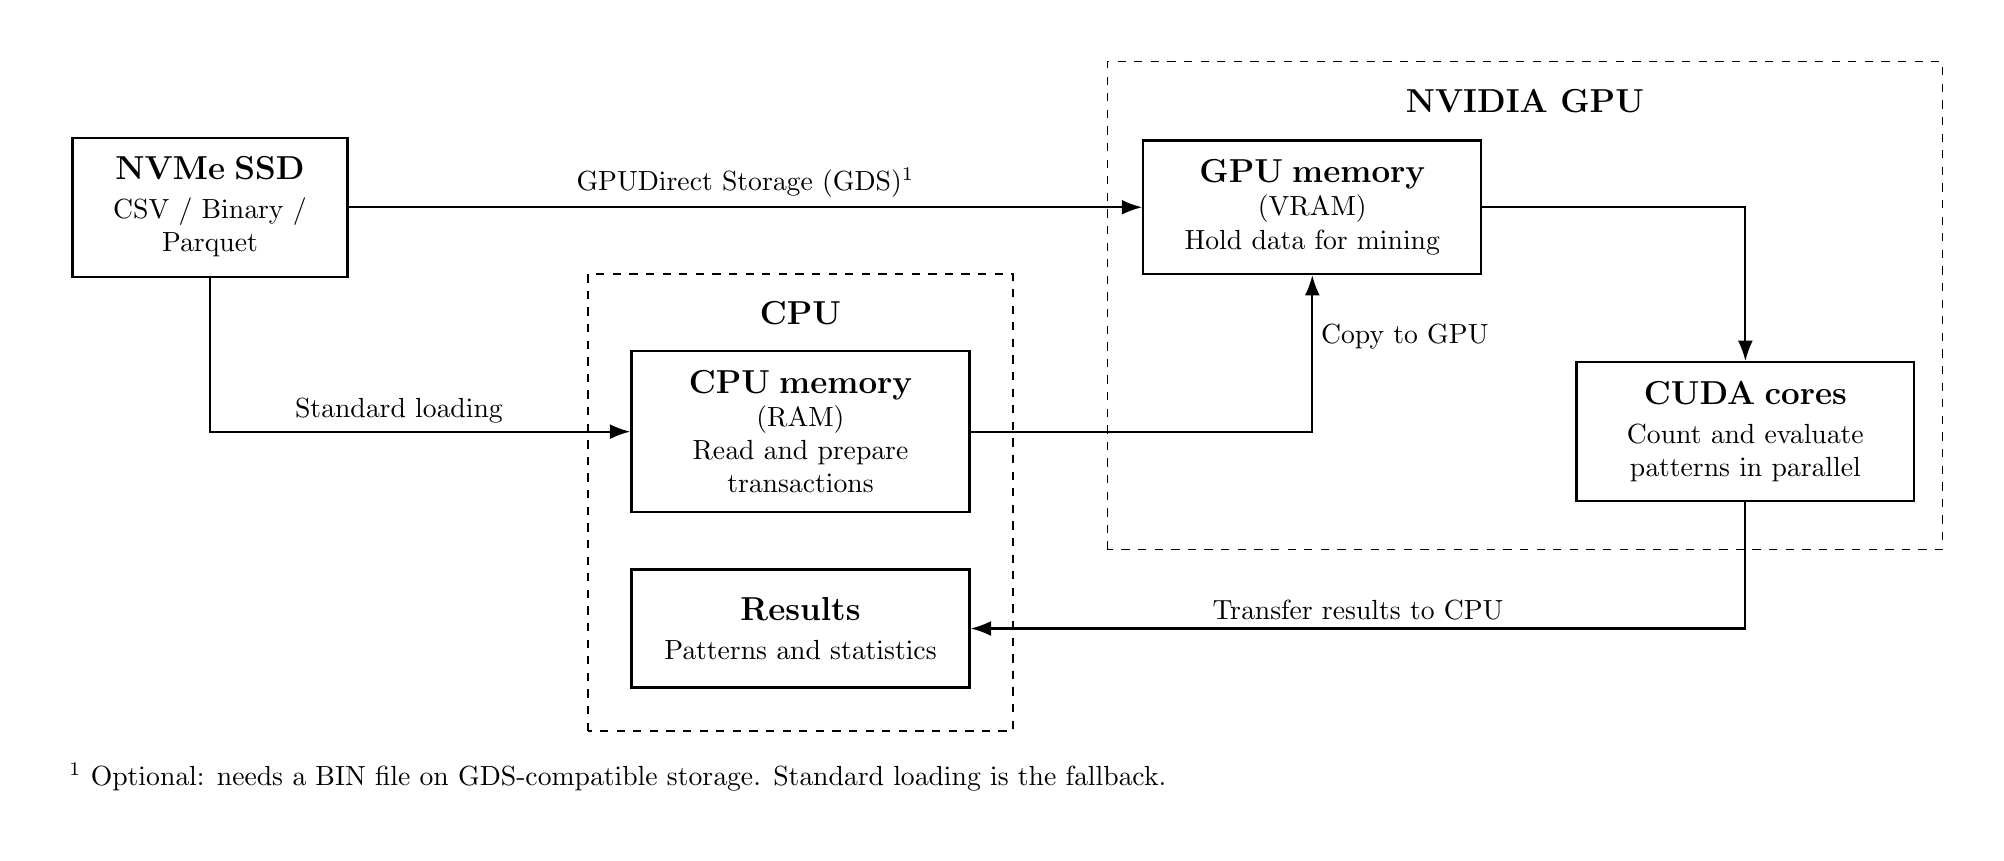
\begin{tikzpicture}[canvas]
% Host and device are physical regions. The direct path runs above the host
% region because it bypasses CPU memory.
\draw[region] (6.4,-1.9) rectangle (11.8,3.9);
\node at (9.1,3.4) {\head{CPU}};
\draw[region] (13.0,.4) rectangle (23.6,6.6);
\node at (18.3,6.1) {\head{NVIDIA GPU}};
\node[box,text width=3cm] (storage) at (1.6,4.75) {\head{NVMe SSD}\\[2pt]\sub{CSV / Binary /\\Parquet}};
\node[box] (host) at (9.1,1.9) {\head{CPU memory}\\\sub{(RAM)\\Read and prepare\\transactions}};
\node[box] (device) at (15.6,4.75) {\head{GPU memory}\\\sub{(VRAM)\\Hold data for mining}};
\node[box] (cores) at (21.1,1.9) {\head{CUDA cores}\\[2pt]\sub{Count and evaluate\\patterns in parallel}};
\node[box] (results) at (9.1,-.6) {\head{Results}\\[2pt]\sub{Patterns and statistics}};
\draw[flow] (storage.east) -- node[note,above] {GPUDirect Storage (GDS)\textsuperscript{1}} (device.west);
\draw[flow] (storage.south) |- (host.west);
\node[note,anchor=south] at (4,1.9) {Standard loading};
\draw[flow] (host.east) -| (device.south);
\node[note,anchor=west] at (15.6,3.1) {Copy to GPU};
\draw[flow] (device.east) -| (cores.north);
\draw[flow] (cores.south) |- node[note,above,pos=.75] {Transfer results to CPU} (results.east);
\node[note,anchor=north west,align=left] at (-.3,-2.2)
 {\textsuperscript{1} Optional: needs a BIN file on GDS-compatible storage. Standard loading is the fallback.};
\end{tikzpicture}
\end{document}
